%!TEX root = ../novoIndex.tex

Considerando a estratégia descrita na solução proposta, os resultados da execução das CNNs aplicadas ao problema de estimação de idade a partir de uma imagem de face são apresentados a seguir. Estes resultados estão organizados segundo abordagens sequenciais, que contemplam desde as técnicas mais elementares, e que vão aumentando o grau de complexidade conforme uso de estratégias específicas da prática de DL para a resolução de problemas práticos.

\section{Abordagem 1: LeNet e AlexNet com Imagens Normalizadas}%sem data augmentation, com normalização e sem equalização

	A primeira abordagem de treinamento considerou o uso dos modelos de maneira canônica, isto é, tais como são definidos na literatura. Adotou-se as funções de ativação não-lineares \emph{ReLU} e \emph{Leaky ReLU} por serem simples de calcular e por satisfazerem os critérios de continuidade e diferenciação, requeridos pelo algoritmo de \emph{backpropagation}, conforme discutido anteriormente na Seção \ref{subsec:modelos}.

	As imagens da base de dados foram normalizadas antes de serem apresentadas às redes. Todos os valores dos pixels componentes das imagens foram escalonados para o intervalo $[0,1]$ por meio de uma divisão por $255$. A prévia normalização das imagens antes da apresentação às CNNs colabora para uma melhor execução do gradiente descendente e diminui a variância nos pesos.

	Os treinamentos destas duas arquiteturas duraram aproximadamente $16$ e $12$ horas respectivamente, em uma instância do Google Compute Engine com 4 CPus virtuais e 15 GB de RAM. Os gráficos de treinamento e as retas zero obtidas a partir da apresentação do conjunto de teste aos modelos consolidados podem ser vistos na Figura \ref{fig:lenet-abordagem1}. É possível notar que ambas as redes sofreram \emph{overfitting} e obtiveram grande margem de erro.

	\begin{figure}[hb!]
		\caption{Resultados do treinamento e teste da CNN LeNet de acordo com a Abordagem 1.}\label{fig:lenet-abordagem1}
	  \begin{subfigure}[hb]{0.5\linewidth}
	    \caption{RMSE de treinamento da arquitetura LeNet utilizando funções de ativação \emph{ReLU}.}
	    \label{fig:redeneuralbiologica}
	    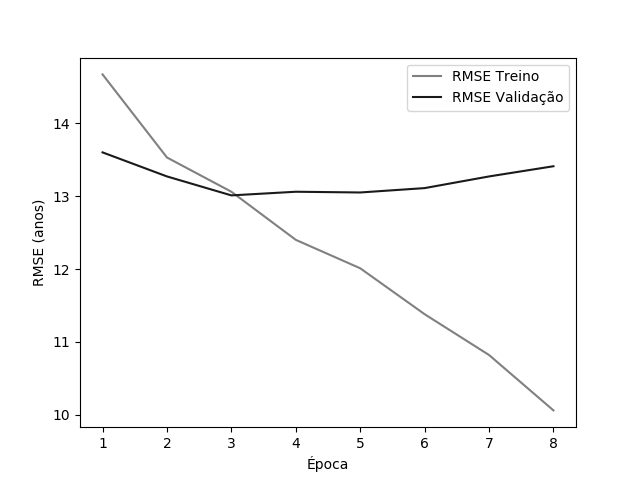
\includegraphics[width=\linewidth]{img/graficos/history/lenet/fig-history-image-treat-1-lenet-relu-rmse.png}%
	  \end{subfigure}%
		\begin{subfigure}[hb]{0.5\linewidth}
			\caption{Reta-0 LeNet \emph{ReLU}.}
			\label{fig:redeneuralbiologica}
			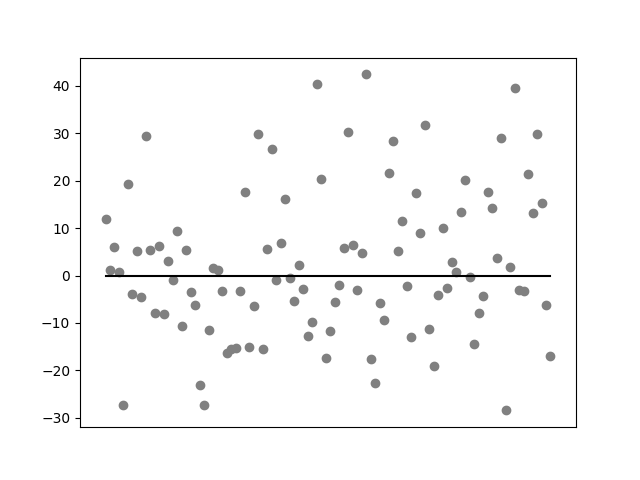
\includegraphics[width=\linewidth]{img/graficos/reta0/lenet/fig-reta-0-image-treat-1-lenet-relu.png}%
		\end{subfigure}\\
	  \begin{subfigure}[hb]{0.5\linewidth}
	    \caption{RMSE de treinamento da arquitetura LeNet utilizando funções de ativação \emph{Leaky ReLU}.}
	    \label{fig:redeneuralbiologica}
	    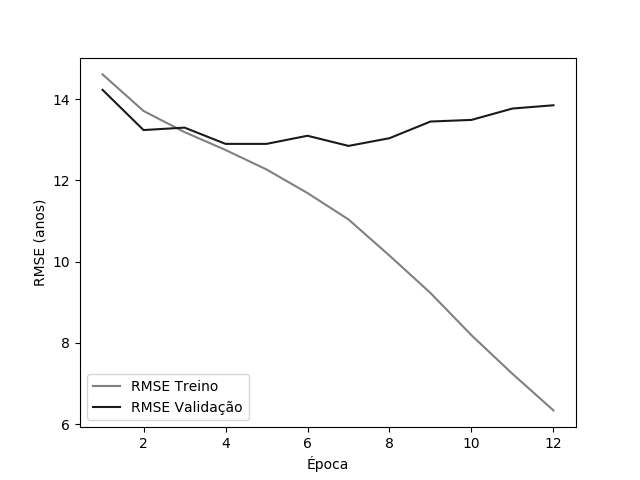
\includegraphics[width=\linewidth]{img/graficos/history/lenet/fig-history-image-treat-1-lenet-lrelu-rmse.png}
	  \end{subfigure}
		\begin{subfigure}[hb]{0.5\linewidth}
			\caption{Reta-0 LeNet \emph{Leaky ReLU}.}
			\label{fig:redeneuralbiologica}
		 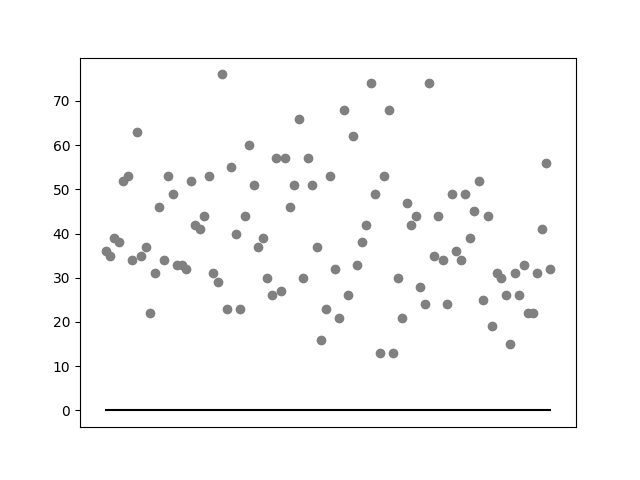
\includegraphics[width=\linewidth]{img/graficos/reta0/lenet/fig-reta-0-image-treat-1-lenet-lrelu.png}
		\end{subfigure}%
	\end{figure}

	\begin{figure}[hb!]
		\caption{Resultados do treinamento e teste da CNN AlexNet de acordo com a Abordagem 1.}\label{fig:alexnet-abordagem1}
		\begin{subfigure}[hb]{0.5\linewidth}
			\caption{Treinamento AlexNet \emph{ReLU}.}
			\label{fig:redeneuralbiologica}
			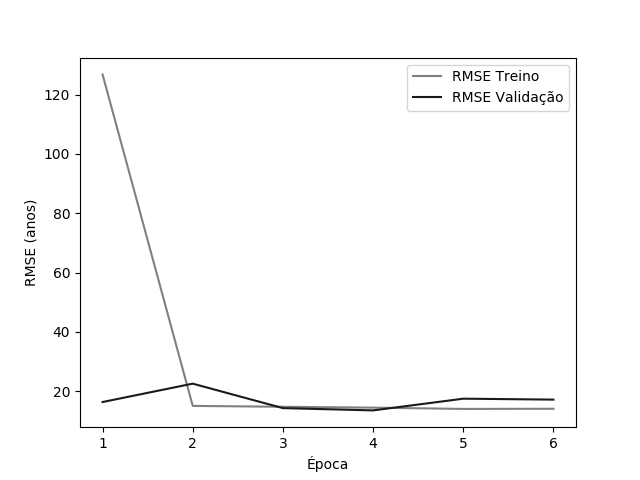
\includegraphics[width=\linewidth]{img/graficos/history/alexnet/fig-history-image-treat-1-alexnet-relu-rmse.png}
		\end{subfigure}
	  \begin{subfigure}[hb]{0.5\linewidth}
	    \caption{Reta-0 AlexNet \emph{ReLU}.}
	    \label{fig:reta0reludying}
	    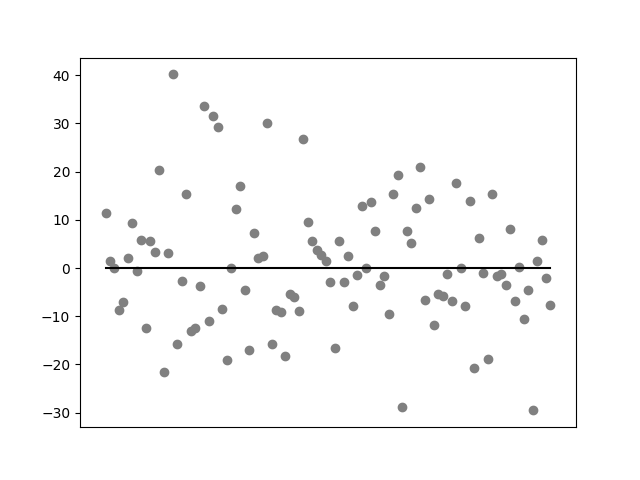
\includegraphics[width=\linewidth]{img/graficos/reta0/alexnet/fig-reta-0-image-treat-1-alexnet-relu.png}%
	  \end{subfigure}\\
		\begin{subfigure}[hb]{0.5\linewidth}
			\caption{Treinamento AlexNet \emph{Leaky ReLU}.}
			\label{fig:histalexlrelunorm}
	    \centering
			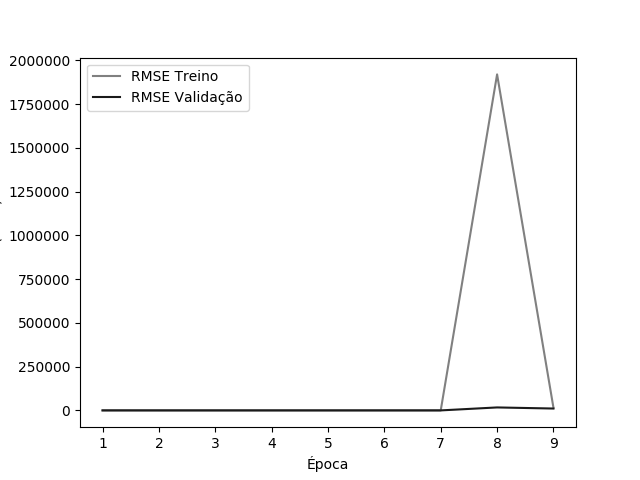
\includegraphics[width=\linewidth]{img/graficos/history/alexnet/fig-history-image-treat-1-alexnet-lrelu-rmse.png}
		\end{subfigure}
	  \begin{subfigure}[hb]{0.5\linewidth}
	    \caption{Reta-0 AlexNet \emph{Leaky ReLU}.}
	    \label{fig:redeneuralbiologica}
	    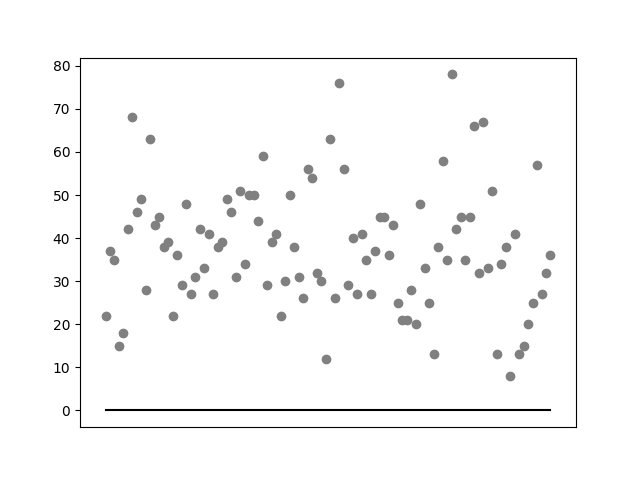
\includegraphics[width=\linewidth]{img/graficos/reta0/alexnet/fig-reta-0-image-treat-1-alexnet-lrelu.png}
	  \end{subfigure}%
	\end{figure}

	Obedecendo ao método de validação cruzada \emph{holdout} previamente mencionado, os resultados desta abordagem encontram-se sintetizados na Tabela \ref{tab:results-1}. É possível constatar que as CNNs com função de ativação \emph{ReLU} obtiveram melhor desempenho, com a arquitetura LeNet, em particular, com resultados ligeiramente superiores.

  \begin{table}[!ht]
		\caption{Resultados do treino e teste dos modelos propostos na Abordagem 1.}
		\label{tab:results-1}
		\begin{center}
			\begin{tabular}{l l l l l}
				\toprule
				Rede & Função de ativação & Épocas & MAE Teste & RMSE Teste \\
				\midrule
				LeNet & \emph{ReLU}  & 4 & 10.53 & 13.55 \\
				LeNet & \emph{Leaky ReLU} & 8 & 38.33 & 40.82 \\
				AlexNet & \emph{ReLU}  & 5 & 11.03 & 13.76 \\
				AlexNet & \emph{Leaky ReLU} & 5 & 39.27 & 41.97 \\
				\bottomrule
			\end{tabular}
		\end{center}
	\end{table}

\section{Abordagem 2: Introduzindo \emph{Data Augmentation}}%com data augmentation, com normalização e sem equalização

	A abordagem anterior consistiu essencialmente da utilização dos modelos tal como foram definidos e com uma simples operação de adequação dos dados de entrada por meio de normalização. Porém, em problemas de Visão Computacional, é comum aplicar técnicas de \emph{data augmentation} com vistas a aumentar artificialmente o conjunto de dados, fazendo com que o modelo, em sua fase de treinamento, não seja exposto à mesma entrada em mais de uma ocasião. Isto previne \emph{overfitting} e colabora para uma melhor generalização \cite{chollet2017deep}.

	As técnicas de \emph{data augmentation} consideradas foram a rotação entre $0$ e $20$ graus no sentido horário ou anti-horário, zoom de $0.8$ a $1.2$ vezes, inversão horizontal com probabilidade de ocorrência de $0.5$ ou translação com probabilidade igual a $0.2$.

	Os gráficos das métricas de desempenho coletadas durante o treinamento e a reta-0 obtida a partir dos dados de teste em cada uma destas quatro configurações são ilustrados nas Figuras \ref{fig:lenet-abordagem2} e \ref{fig:alexnet-abordagem2}.

	\begin{figure}[h!]
		\caption{Resultados do treinamento e teste da CNN LeNet de acordo com a Abordagem 2.}\label{fig:lenet-abordagem2}
		\begin{subfigure}[hb]{0.5\linewidth}
			\caption{RMSE de treinamento da arquitetura LeNet utilizando funções de ativação \emph{ReLU}.}
			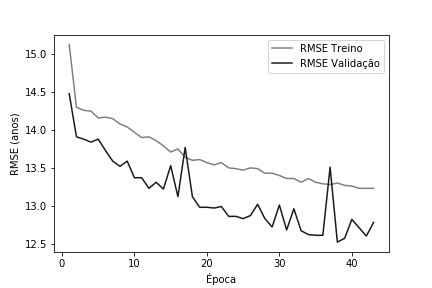
\includegraphics[width=\linewidth]{img/graficos/history/lenet/fig-history-image-treat-2-lenet-relu-rmse.png}%
		\end{subfigure}%
		\begin{subfigure}[hb]{0.5\linewidth}
			\caption{Reta-0 LeNet \emph{ReLU}.}
			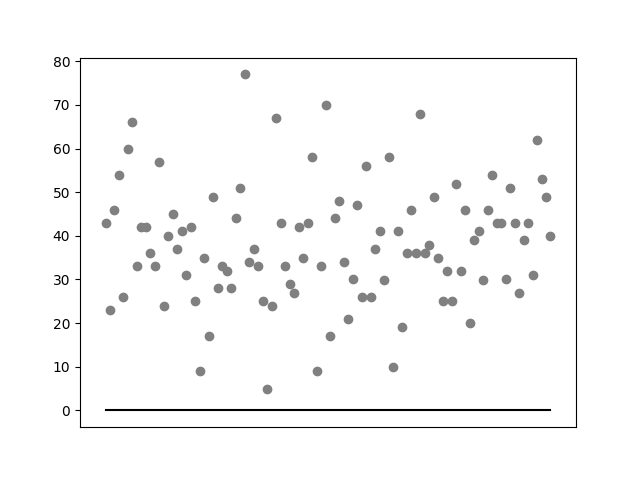
\includegraphics[width=\linewidth]{img/graficos/reta0/lenet/fig-reta-0-image-treat-2-lenet-relu.png}%
		\end{subfigure}\\
		\begin{subfigure}[hb]{0.5\linewidth}
			\caption{RMSE de treinamento da arquitetura LeNet utilizando funções de ativação \emph{Leaky ReLU}.}
			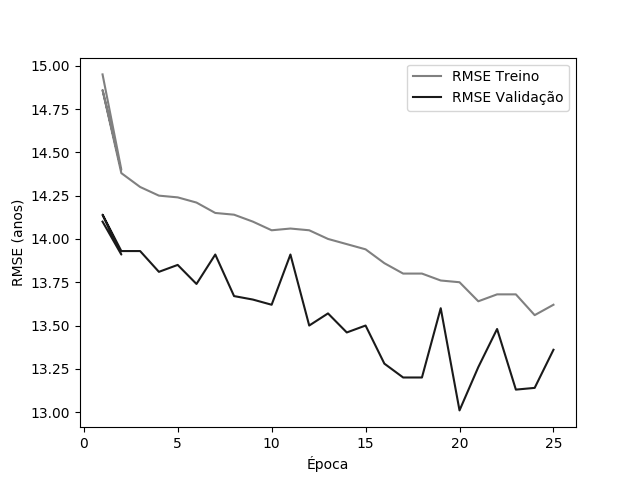
\includegraphics[width=\linewidth]{img/graficos/history/lenet/fig-history-image-treat-2-lenet-lrelu-rmse.png}
		\end{subfigure}
		\begin{subfigure}[hb]{0.5\linewidth}
			\caption{Reta-0 LeNet \emph{Leaky ReLU}.}
		 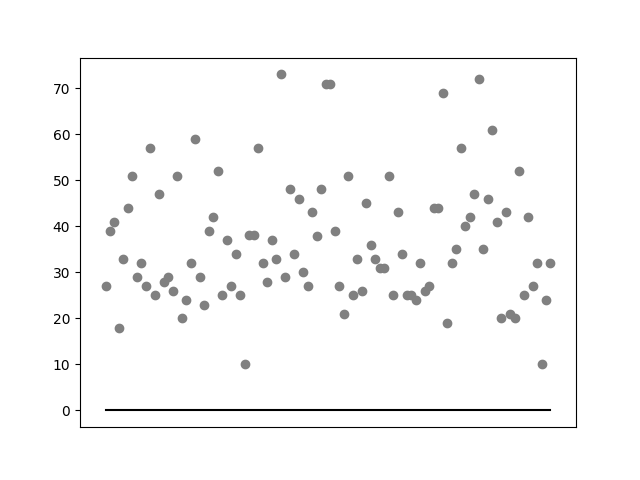
\includegraphics[width=\linewidth]{img/graficos/reta0/lenet/fig-reta-0-image-treat-2-lenet-lrelu.png}
		\end{subfigure}%
	\end{figure}

	\begin{figure}[h!]
		\caption{Resultados do treinamento e teste da CNN AlexNet de acordo com a Abordagem 2.}\label{fig:alexnet-abordagem2}
		\begin{subfigure}[hb]{0.5\linewidth}
			\caption{Treinamento AlexNet \emph{ReLU}.}
			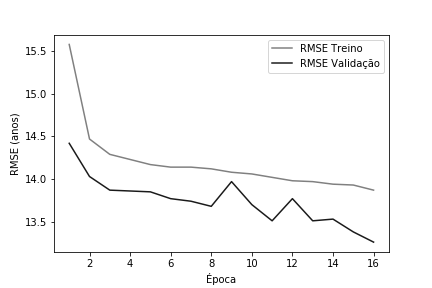
\includegraphics[width=\linewidth]{img/graficos/history/alexnet/fig-history-image-treat-2-alexnet-relu-rmse.png}
		\end{subfigure}
		\begin{subfigure}[hb]{0.5\linewidth}
			\caption{Reta-0 AlexNet \emph{ReLU}.}
			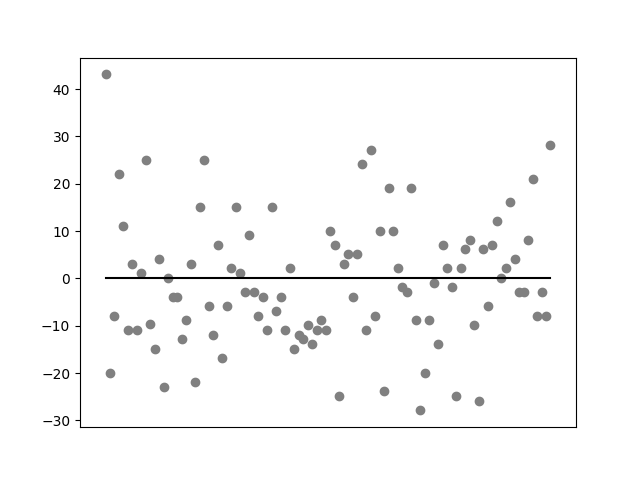
\includegraphics[width=\linewidth]{img/graficos/reta0/alexnet/fig-reta-0-image-treat-2-alexnet-relu.png}%
		\end{subfigure}\\
		\begin{subfigure}[hb]{0.5\linewidth}
			\caption{Treinamento AlexNet \emph{Leaky ReLU}.}
			\centering
			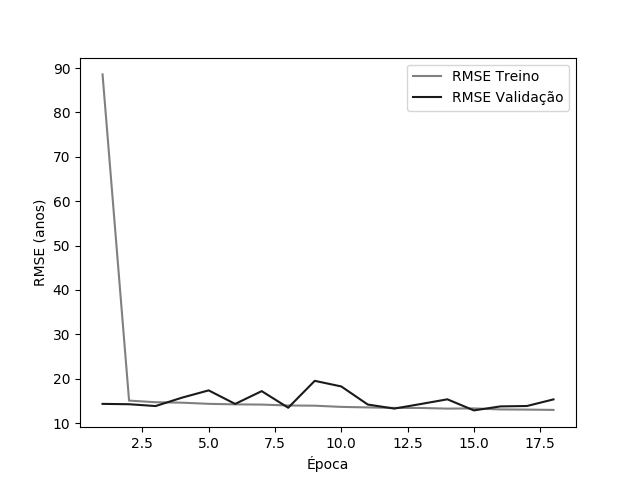
\includegraphics[width=\linewidth]{img/graficos/history/alexnet/fig-history-image-treat-2-alexnet-lrelu-rmse.png}
		\end{subfigure}
		\begin{subfigure}[hb]{0.5\linewidth}
			\caption{Reta-0 AlexNet \emph{Leaky ReLU}.}
			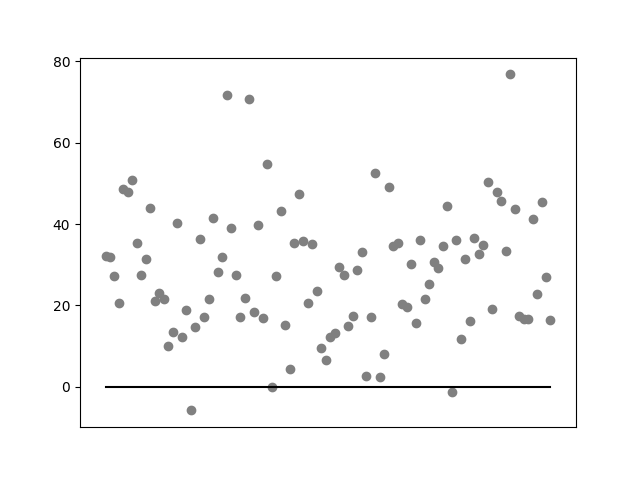
\includegraphics[width=\linewidth]{img/graficos/reta0/alexnet/fig-reta-0-image-treat-2-alexnet-lrelu.png}
		\end{subfigure}%
	\end{figure}

	De maneira análoga, as métricas de desempenho coletadas encontram-se detalhadas na Tabela \ref{tab:results2}. Nota-se que o número de épocas no treinamento foi maior que a abordagem anterior, indicando que houve um cenário mais favorável para o aprendizado dos padrões nos dados. De maneira geral, as métricas obtidas não fornecem uma evidência forte de que esta segunda abordagem produz resultados mais significativos que a primeira mas, no caso da CNN AlexNet com \emph{ReLU}, os resultados foram comparáveis.

	\begin{table}[!ht]
		\caption{Resultados do treino e teste dos modelos propostos na Abordagem 2.}
		\label{tab:results2}
		\begin{center}
			\begin{tabular}{l l l l l}
				\toprule
				Rede & Função de ativação & Épocas & MAE Teste & RMSE Teste \\
				\midrule
				LeNet & \emph{ReLU}  & 39 & 37.85 & 40.27 \\
				LeNet & \emph{Leaky ReLU} & 21 & 38.50 & 41.06 \\
				AlexNet & \emph{ReLU}  & 16 & 11.59 & 14.59 \\
				AlexNet & \emph{Leaky ReLU} & 16 & 28.06 & 31.81 \\
				\bottomrule
			\end{tabular}
		\end{center}
	\end{table}

	O efeito positivo esperado pelo \emph{data augmentation} não se mostrou tão evidente quanto se esperava inicialmente. Porém, isto pode acontecer em razão dos valores dos hiperparâmetros e da necessidade de melhor pré-processamento das imagens antes da apresentação às CNNs, o que motivou a realização da abordagem a seguir.

\section{Abordagem 3: Introduzindo Equalização de Histograma}%com data augmentation, com normalização e com equalização
	A terceira abordagem utilizou as imagens da base de dados normalizadas e técnicas de \emph{data augmentation} previamente mencionadas. Considerando os resultados obtidos na abordagem anterior, introduziu-se o processo de equalização das imagens por histograma, que ajusta o contraste da imagem utilizando o histograma de cores. Este método aumenta o contraste global de imagens, especialmente quando os dados úteis da imagem são representados por cores próximas. Isto faz com que áreas de contraste menor ganhem mais contraste. No contexto da detecção de idade por meio da imagem da face de determinado indivíduo, a equalização por histograma reforça marcas de expressões e outras imperfeições \cite{acharya2005image}. %É possivel observar na Figura \ref{} uma imagem do conjunto de dados original e após o processo de equalização por histograma.

	A partir desta abordagem foran obtidos os gráficos de trenamento e a reta-0 das redes LeNet e AlexNet, que estão nas Figuras \ref{fig:lenet-abordagem3} e \ref{fig:alexnet-abordagem3}, respectivamente.

	\begin{figure}[hb!]
		\caption{Resultados do treinamento e teste da CNN LeNet de acordo com a Abordagem 3.}\label{fig:lenet-abordagem3}
		\begin{subfigure}[hb]{0.5\linewidth}
			\caption{RMSE de treinamento da arquitetura LeNet utilizando funções de ativação \emph{ReLU}.}
			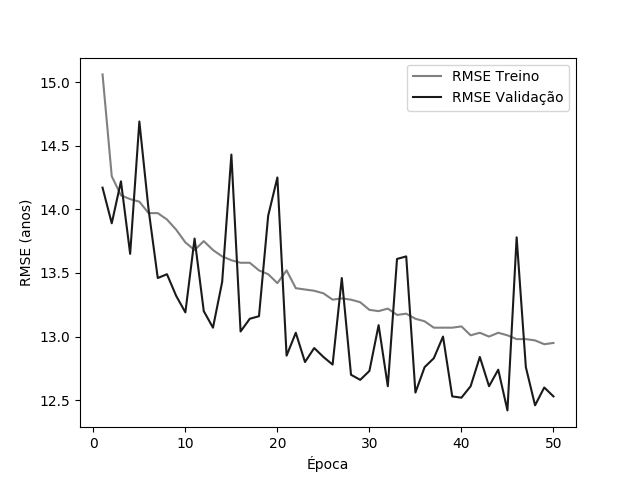
\includegraphics[width=\linewidth]{img/graficos/history/lenet/fig-history-image-treat-3-lenet-relu-rmse.png}%
		\end{subfigure}%
		\begin{subfigure}[hb]{0.5\linewidth}
			\caption{Reta-0 LeNet \emph{ReLU}.}
			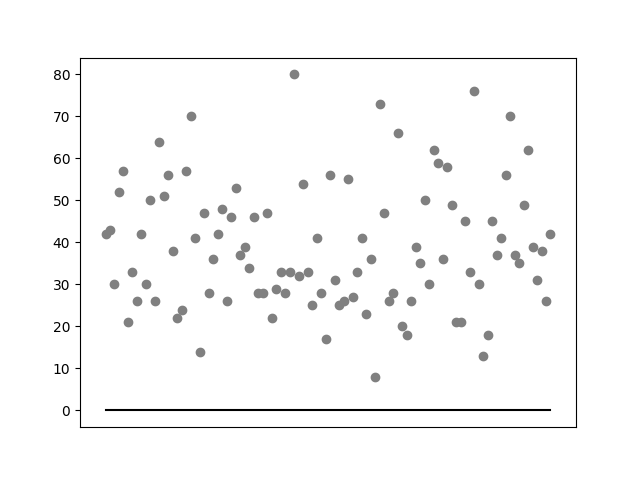
\includegraphics[width=\linewidth]{img/graficos/reta0/lenet/fig-reta-0-image-treat-3-lenet-relu.png}%
		\end{subfigure}\\
		\begin{subfigure}[hb]{0.5\linewidth}
			\caption{RMSE de treinamento da arquitetura LeNet utilizando funções de ativação \emph{Leaky ReLU}.}
			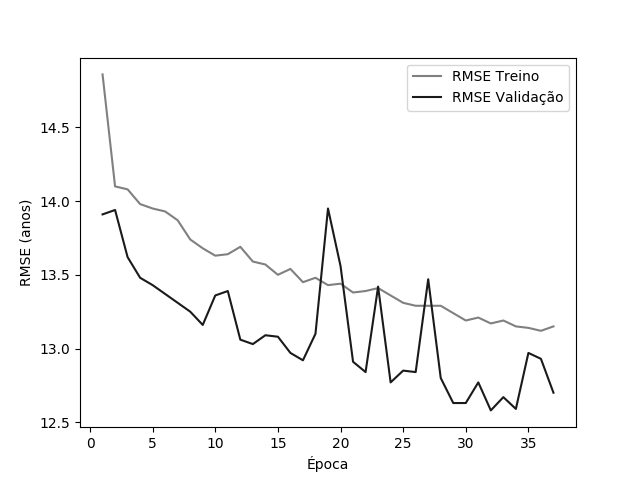
\includegraphics[width=\linewidth]{img/graficos/history/lenet/fig-history-image-treat-3-lenet-lrelu-rmse.png}
		\end{subfigure}
		\begin{subfigure}[hb]{0.5\linewidth}
			\caption{Reta-0 LeNet \emph{Leaky ReLU}.}
		 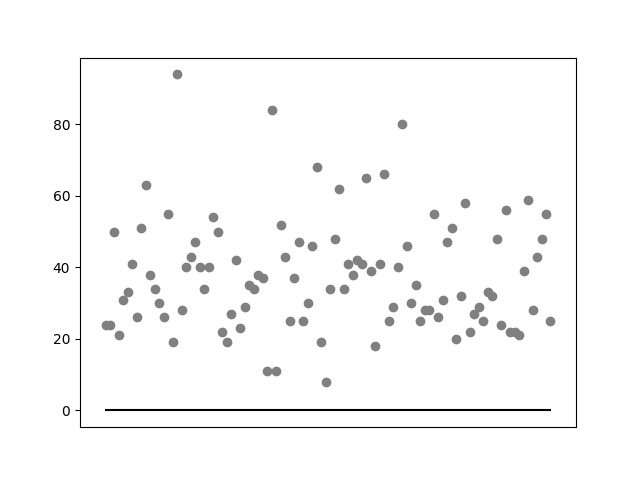
\includegraphics[width=\linewidth]{img/graficos/reta0/lenet/fig-reta-0-image-treat-3-lenet-lrelu.png}
		\end{subfigure}%
	\end{figure}

	\begin{figure}[hb!]
		\caption{Resultados do treinamento e teste da CNN AlexNet de acordo com a Abordagem 3.}\label{fig:alexnet-abordagem3}
		\begin{subfigure}[hb]{0.5\linewidth}
			\caption{RMSE de treinamento da arquitetura AlexNet utilizando funções de ativação \emph{ReLU}.}
			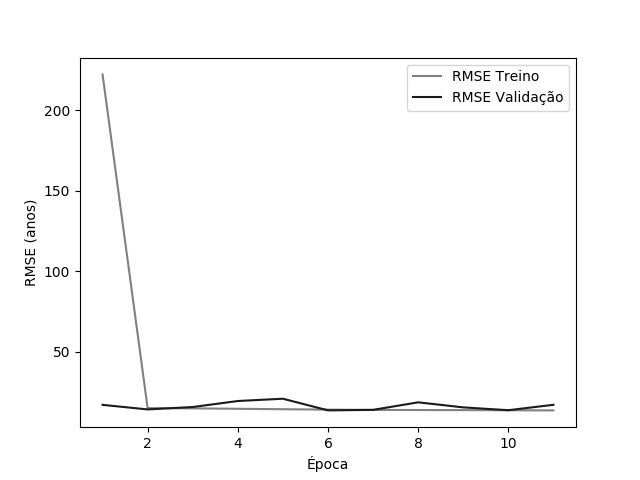
\includegraphics[width=\linewidth]{img/graficos/history/alexnet/fig-history-image-treat-3-alexnet-relu-rmse.png}
		\end{subfigure}
		\begin{subfigure}[hb]{0.5\linewidth}
			\caption{Reta-0 AlexNet \emph{ReLU}.}
			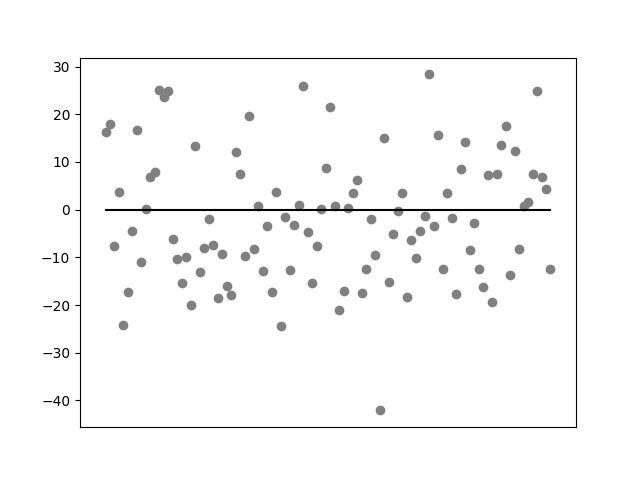
\includegraphics[width=\linewidth]{img/graficos/reta0/alexnet/fig-reta-0-image-treat-3-alexnet-relu.png}%
		\end{subfigure}\\
		\begin{subfigure}[hb]{0.5\linewidth}
			\caption{RMSE de treinamento da arquitetura AlexNet utilizando funções de ativação RMSE de treinamento da arquitetura LeNet utilizando funções de ativação \emph{Leaky ReLU}.}
			\centering
			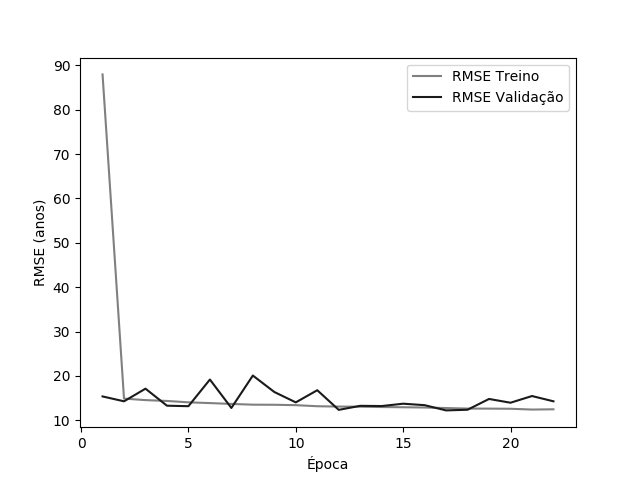
\includegraphics[width=\linewidth]{img/graficos/history/alexnet/fig-history-image-treat-3-alexnet-lrelu-rmse.png}
		\end{subfigure}
		\begin{subfigure}[hb]{0.5\linewidth}
			\caption{Reta-0 AlexNet \emph{Leaky ReLU}.}
			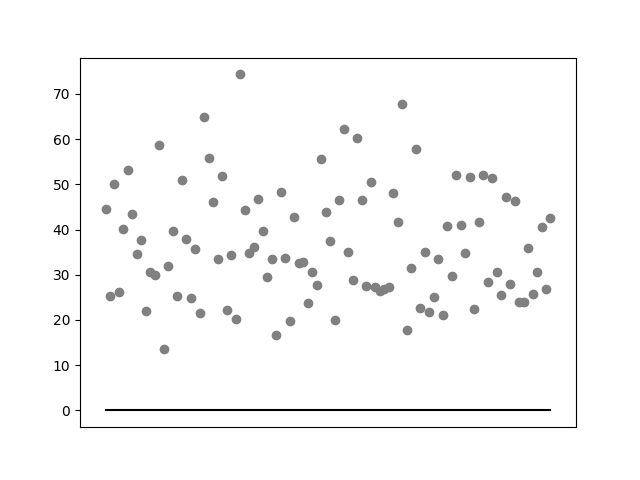
\includegraphics[width=\linewidth]{img/graficos/reta0/alexnet/fig-reta-0-image-treat-3-alexnet-lrelu.png}
		\end{subfigure}%
	\end{figure}

	Obedecendo ao método de validação cruzada \emph{holdout} previamente mencionado, os resultados desta abordagem encontram-se sintetizados na Tabela \ref{tab:results-3}.

	\begin{table}[!ht]
		\caption{Resultados do treino e teste dos modelos propostos na Abordagem 3.}
		\label{tab:results-3}
		\centering
		\begin{tabular}{l l l l l l l}
				\toprule
				Rede & Função de ativação & Épocas & MAE Teste & RMSE Teste \\
				\midrule
				LeNet & \emph{ReLU} & 46 &  38.66 & 41.20 \\
				LeNet & \emph{Leaky ReLU} &  38 & 38.26 & 40.85 \\
				AlexNet & \emph{ReLU} & 7 & 13.10 & 15.88 \\
				AlexNet & \emph{Leaky ReLU} & 18 & 35.25 & 38.04 \\
				\bottomrule
			\end{tabular}
	\end{table}

\section{Abordagem 4: Utilizando MAE para o cálculo da perda}%com data augmentation, com normalização e com equalização, usando mae pra loss
	A análise dos gráficos de treinamento das redes anteriores levou à suposição de que a métrica utilizada para a atualização dos pesos RMSE estivesse trazendo instabilidade para o treinamento. Desta maneira, esta abordagem considera o treinamento da rede LeNet com \emph{data augmentation}, imagens normalizadas e com equalização por histograma, utilizando MAE para cálculo da perda. Os gráficos do treinamento e reta-0 desta abordagem estão nas Figuras \ref{fig:lenet-abordagem4}.

	\begin{figure}[hb!]
		\caption{Resultados do treinamento e teste da CNN LeNet de acordo com a Abordagem 4.}\label{fig:lenet-abordagem4}
		\begin{subfigure}[hb]{0.5\linewidth}
			\caption{MAE de treinamento da arquitetura LeNet utilizando funções de ativação \emph{ReLU}.}
			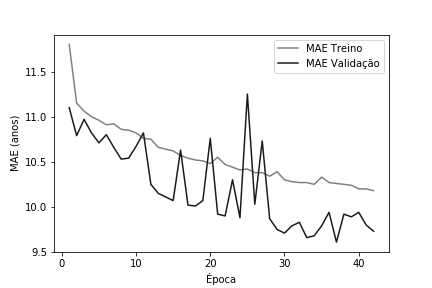
\includegraphics[width=\linewidth]{img/graficos/history/lenet/fig-history-abordagem-4-lenet-relu-mae.png}%
		\end{subfigure}%
		\begin{subfigure}[hb]{0.5\linewidth}
			\caption{Reta-0 LeNet \emph{ReLU}.}
			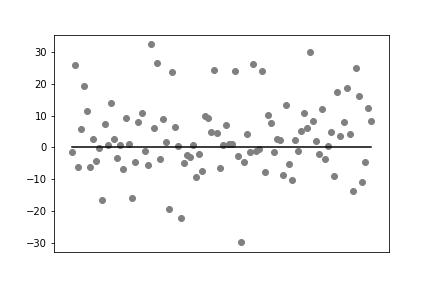
\includegraphics[width=\linewidth]{img/graficos/reta0/lenet/fig-reta-0-abordagem-4-lenet-relu.png}%
		\end{subfigure}\\
	\end{figure}

	Obedecendo ao método de validação cruzada \emph{holdout} previamente mencionado, os resultados desta abordagem encontram-se sintetizados na Tabela \ref{tab:results-4}.

	\begin{table}[!ht]
		\centering
		\caption{Resultados do treino e teste dos modelos propostos na Abordagem 4.}
		\label{tab:results-4}
			\begin{tabular}{l l l l l l l}
				\toprule
				Rede & Função de ativação & Épocas & MAE Teste & RMSE Teste \\
				\midrule
				LeNet & \emph{Leaky ReLU} & 38 & 9.98 & 12.91 \\
				\bottomrule
			\end{tabular}
	\end{table}

	É possível notar que esta abordagem trouxe métrocas de desempenho mais satisfatórias que as obtidas até então. Porém, as escolhas da rede, função de ativação e pré-processamento de imagens de entrada foram feitas a partir do palpite de que \emph{data augmentation} e equalização por histograma trariam redes mais fortes. Assim, há a necessidade de verificar o desempenho de uma rede similar, porém sem estes processos.

\section{Abordagem 5: Rede com melhor desempenho}% sem data augmentation, com normalização e sem equalização, usando mae pra loss, batch de 128, sem patience
	A quinta abordagem adotou a rede com melhor desempenho obtido até o momento. Neste caso, considerou-se a rede LeNet treinada com imagens da base de dados normalizadas, mas sem equalização de histograma de cores ou técnicas de \emph{data augmentation}. Seguiu-se utilizando a métrica MAE para o cálculo da perda e da atualização dos pesos. Buscando garantir maior estabilidade nas métricas de desempenho durante o treinamento, aumentou-se o tamanho do batch para 128, haja vista a característica instável do treinamento mostrada nas abordagens anteriores.

	\begin{figure}[hb!]
		\caption{Resultados do treinamento e teste da CNN LeNet de acordo com a Abordagem 5.}\label{fig:lenet-abordagem5}
		\begin{subfigure}[hb]{0.5\linewidth}
			\caption{MAE de treinamento da arquitetura LeNet utilizando funções de ativação \emph{ReLU}.}
			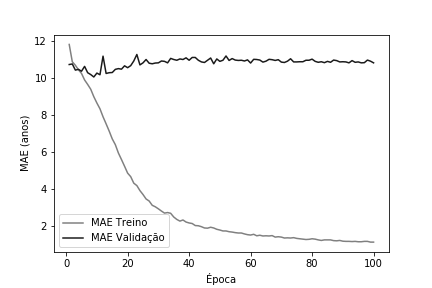
\includegraphics[width=\linewidth]{img/graficos/history/lenet/fig-history-abordagem-5-lenet-relu-mae.png}%
		\end{subfigure}%
		\begin{subfigure}[hb]{0.5\linewidth}
			\caption{Reta-0 LeNet \emph{ReLU}.}
			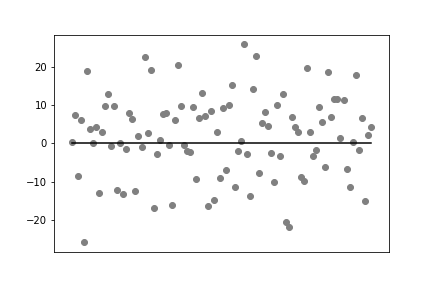
\includegraphics[width=\linewidth]{img/graficos/reta0/lenet/fig-reta-0-abordagem-5-lenet-relu.png}%
		\end{subfigure}\\
	\end{figure}

	Obedecendo ao método de validação cruzada \emph{holdout} previamente mencionado, os resultados desta abordagem encontram-se sintetizados na Tabela \ref{tab:results-5}.

	\begin{table}[!ht]
		\centering
		\caption{Resultados do treino e teste dos modelos propostos na Abordagem 5.}
		\label{tab:results-5}
			\begin{tabular}{l l l l l l l}
				\toprule
				Rede & Função de ativação & Épocas & MAE Teste & RMSE Teste \\
				\midrule
				LeNet & \emph{ReLU} & 9 &  10.09 & 13.04 \\
				\bottomrule
			\end{tabular}
		\end{table}


\section{Abordagem 6: VGG-16}
	Após a utilização exaustiva de redes mais simples, decidiu-se por utilizar uma rede canônica mais extensa. A VGG-16, detalhada na Seção \ref{sec:canonicos} \todo{add label}, foi treinada sem utilizar técnicas de \emph{transfer learning}. Removeu-se a última camada, responsável pela classificação, e adicionou-se uma camada densa com função de ativação ReLU. Os resultados obtidos estão na Figura \ref{fig:vgg-abordagem6}.

		\begin{figure}[hb!]
			\caption{Resultados do treinamento e teste da CNN VGG-16 de acordo com a Abordagem 6.}\label{fig:vgg-abordagem6}
			\begin{subfigure}[hb]{0.5\linewidth}
				\caption{MAE de treinamento da arquitetura VGG-16 utilizando funções de ativação \emph{ReLU}.}
				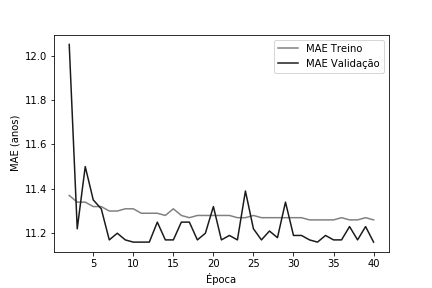
\includegraphics[width=\linewidth]{img/graficos/history/vgg16/fig-history-abordagem6-vgg16-relu-mae.png}%
			\end{subfigure}%
			\begin{subfigure}[hb]{0.5\linewidth}
				\caption{Reta-0 LeNet \emph{ReLU}.}
				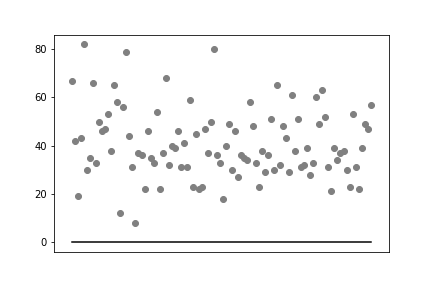
\includegraphics[width=\linewidth]{img/graficos/reta0/vgg16/fig-reta-0-abordagem6-vgg16-relu.png}%
			\end{subfigure}\\
		\end{figure}

\begin{table}[!ht]
	\centering
	\caption{Resultados do treino e teste dos modelos propostos na Abordagem 6.}
	\label{tab:results-2}
		\begin{tabular}{l l l l l l l}
			\toprule
			Rede & Função de ativação & Épocas & MAE Teste & RMSE Teste \\
			\midrule
			%%LeNet & \emph{ReLU} & 9 &  10.09 & 13.04 \\
			\bottomrule
		\end{tabular}
	\end{table}
	Observa-se que a rede foi vítima de \emph{Dying ReLU problem}. Com o objetivo de contornar este problema, decidiu-se utilizar \emph{Data Augmentation} e normalização por histograma de frequência.

\section{Abordagem 7: VGG-16 com Data Augmentation}

	A rede VGG-16 foi instanciada e treinada utilizando os mesmos parâmetros descritos na Abordagem 6. Porém, passou-se a utilizar \emph{Data Augmentation}, repetindo-se a configuração utilziada nas Abordagens 3 e 4.

		\begin{figure}[hb!]
			\caption{Resultados do treinamento e teste da CNN VGG-16 de acordo com a Abordagem 7.}\label{fig:vgg-abordagem6}
			\begin{subfigure}[hb]{0.5\linewidth}
				\caption{MAE de treinamento da arquitetura VGG-16 utilizando funções de ativação \emph{ReLU}.}
				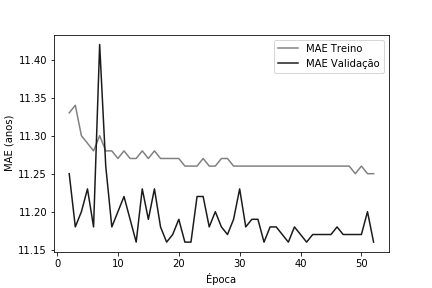
\includegraphics[width=\linewidth]{img/graficos/history/vgg16/fig-history-abordagem7-vgg16-relu-mae.png}%
			\end{subfigure}%
			\begin{subfigure}[hb]{0.5\linewidth}
				\caption{Reta-0 LeNet \emph{ReLU}.}
				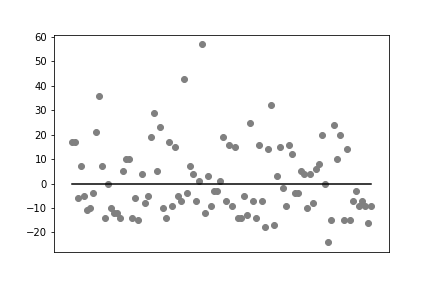
\includegraphics[width=\linewidth]{img/graficos/reta0/vgg6/fig-reta-0-abordagem7-vgg16-relu.png}%
			\end{subfigure}\\
		\end{figure}

\begin{table}[!ht]
	\centering
	\caption{Resultados do treino e teste dos modelos propostos na Abordagem 6.}
	\label{tab:results-2}
		\begin{tabular}{l l l l l l l}
			\toprule
			Rede & Função de ativação & Épocas & MAE Teste & RMSE Teste \\
			\midrule
			%%LeNet & \emph{ReLU} & 9 &  10.09 & 13.04 \\
			\bottomrule
		\end{tabular}
	\end{table}
	Observa-se que a rede foi vítima de \emph{Dying ReLU problem}. Com o objetivo de contornar este problema, decidiu-se utilizar \emph{Data Augmentation} e normalização por histograma de frequência.



\section{Abordagem 8: VGG-16 com Leaky ReLU e taxa de aprendizado de $0.003$}


\section{Abordagem 9: SqueezeNet}
